\section{Results}

\subsection{Seq2Seq and Transformer models}
Both the Seq2Seq and Transformer models seem to train slowly due to the large amount of data provided.

While we were not able to train many epochs due to technical reasons, this didn't seem to be necessary as both models have a minimal loss at epochs 11 and 14, respectively.

\begin{figure}[h]
	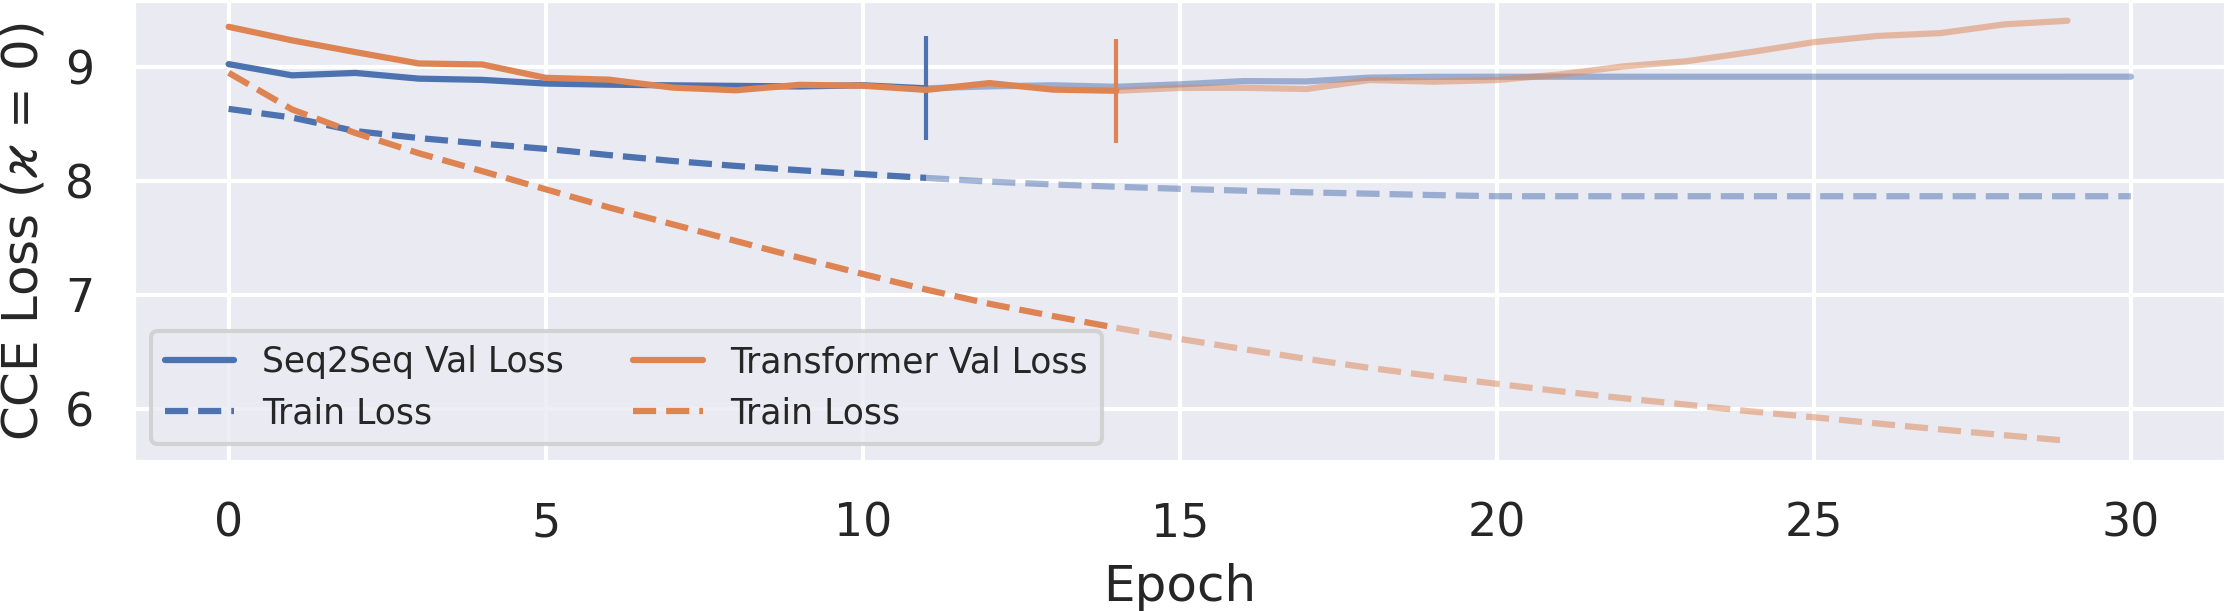
\includegraphics[width = \textwidth]{baseline_losses.png}
	\caption{Training and validation losses of both initial models. Due to early stopping, only the non-transparent part is considered.}
\end{figure}

While the categorical cross-entropy loss of these models seems similar, their ROUGE scores tell another story.
\Cref{baseline_rouges} contains the ROUGE-1 and ROUGE-2 scores of both models, where the transformer produces a considerably better score.

\begin{figure}[h]
	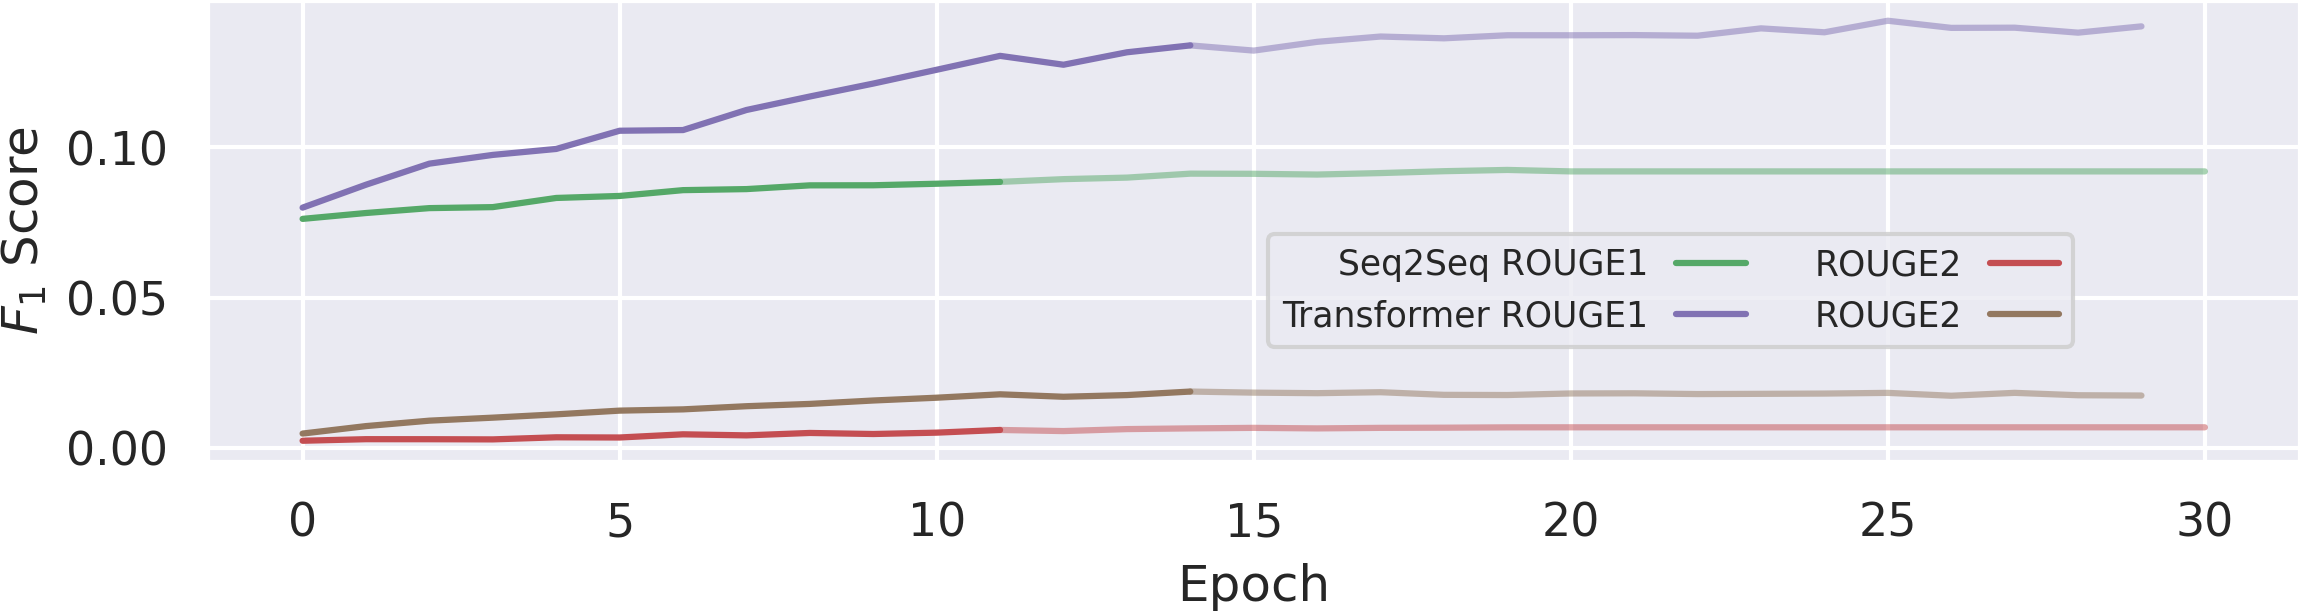
\includegraphics[width = \textwidth]{baseline_rouges.png}
	\caption{ROUGE scores of the Seq2Seq and Transformer models. The attention mechanism allows the transformer model to create more coherent result with higher ROUGE scores.}
	\label{baseline_rouges}
\end{figure}

Are these relatively good ROUGE scores good for having reasonable results?
The answer is a resounding \textbf{NO}.

\Cref{seq2seq_example,transformer_example} in \appendixA show some examples of the outputs from this model.
The results are nonsensical, and there is nothing that could even suggest where to start.

\subsection{BERTFormer}

With its pre-trained encoder, the BERTFormer model produced a better result than the regular Transformer model in both ROUGE scores.
However, it also gets to the best validation loss early, at epoch 12.

\begin{figure}[h]
	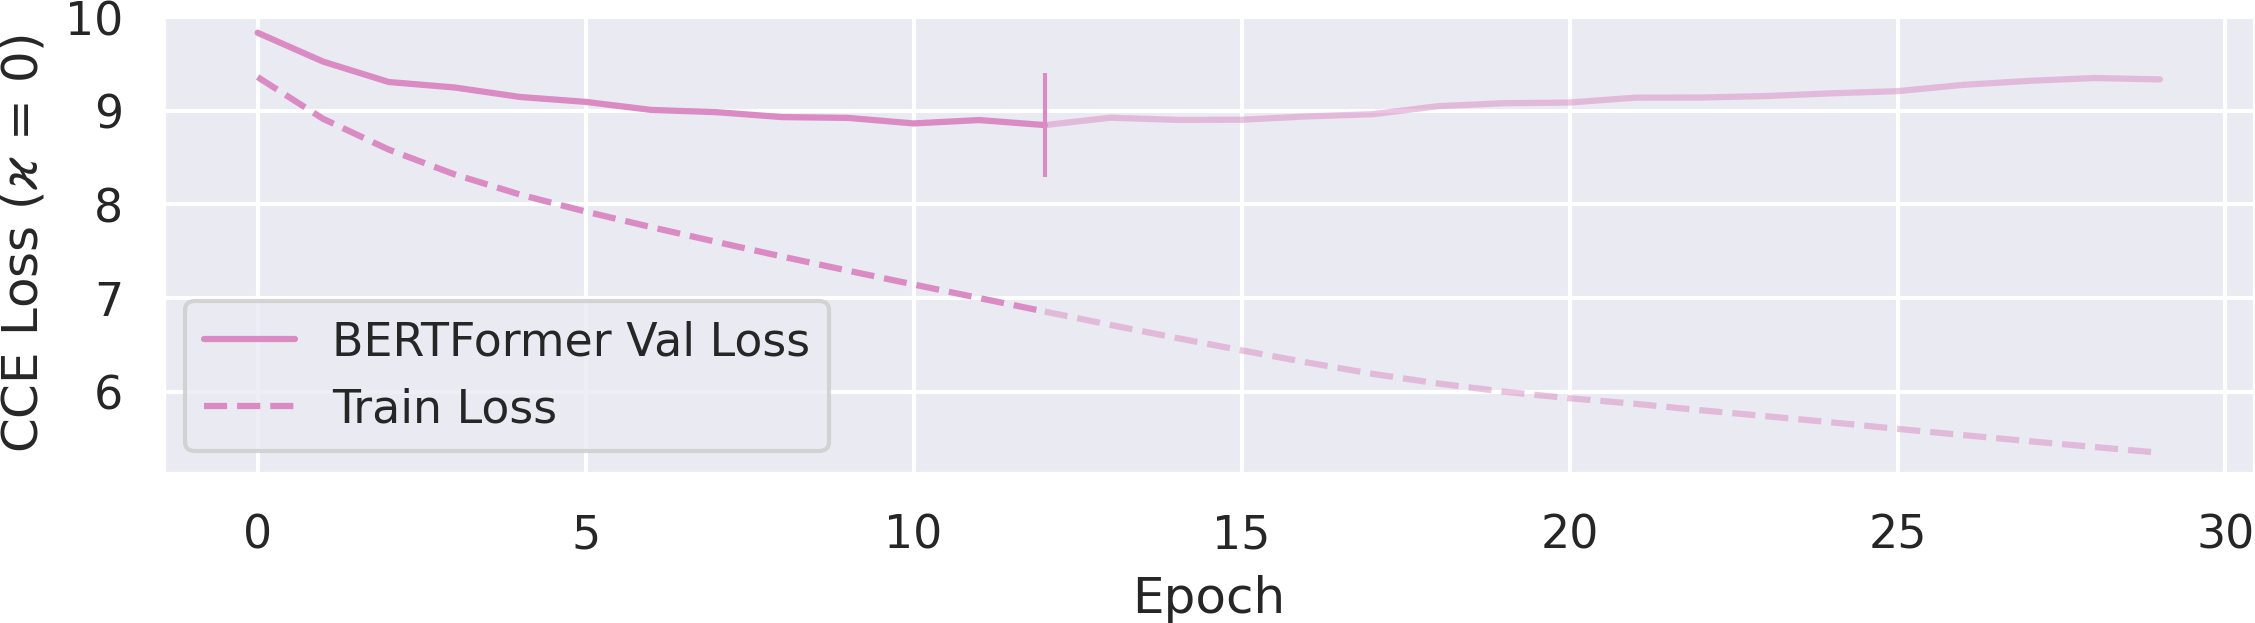
\includegraphics[width=\textwidth]{bertformer_loss.png}
	\caption{Training and validation loss of the BERTFormer transformer. It's notable that there is little change in the validation loss between epochs; this is likely an unfortunate artifact of the embeddings and the decoder of the classifier not learning much and categorical cross-entropy not being a good loss to minimise for this problem.}
\end{figure}

Despite this, it has significantly better ROUGE scores than the previous two classifiers, as can be seen in \cref{comparison_table}.

\begin{figure}[h]
	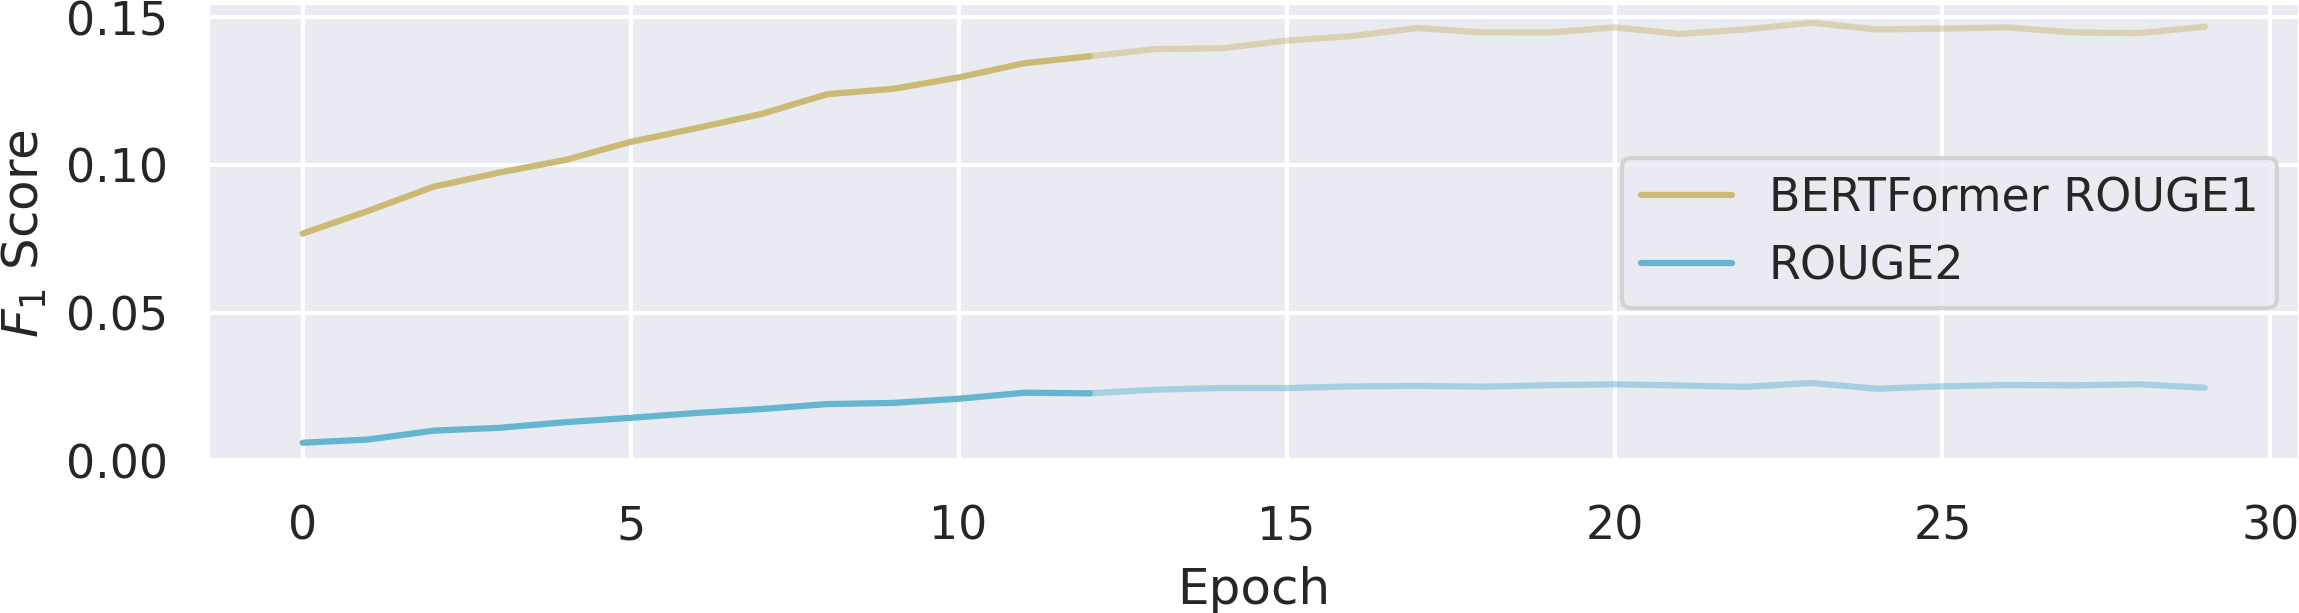
\includegraphics[width=\textwidth]{bertformer_rouge.png}
	\caption{ROUGE-1 and ROUGE-2 scores of the BERTFormer transformer, as it trains. The Rouge-1 score grows rapidly after the CCE loss stops growing and the training stops early; this is another proof that this loss might not be the best for this problem.}
\end{figure}

\begin{table}[h]
	\centering
	\footnotesize
	\begin{tabular}{l | c c c}
		\toprule
			Model & CCE & ROUGE-1 & ROUGE-2 \\
		\midrule
			Seq2Seq & 8.809 & 0.088 & 0.006 \\
			Transformer & 8.787 & 0.134 & 0.019 \\
			BERTFormer & 8.846 & 0.137 & 0.023 \\
		\bottomrule
	\end{tabular}
	\caption{Comparison of final scores between models. See \appendixA{} for the tragically bad actual results.}
	\label{comparison_table}
\end{table}

Sadly, this model keeps giving nonsensical and unworkable results, as seen in \cref{bertformer_example} in \appendixA{}
